%
% Chapter 7 - Schedule
%
\chapter{Schedule} \label{cap:schedule}

The final project timeline is presented in the Gantt chart in Figure~\ref{fig:schedule}. It tracks three primary tracks, Deliverables, Backend, and Frontend, together with two continuous activities that spanned the entire project lifecycle. All planned tasks were completed on schedule.

\begin{itemize}
    \item \textbf{Continuous activities:} reporting and testing ran throughout the project, from its start on March 13th, 2026, through to the final submission, ensuring documentation and system stability were maintained alongside development.
    \item \textbf{Deliverables and milestones:} the Initial Report was delivered on March 13th, 2026, the Intermediate Report on May 1st, 2026, and this Final Report concludes the project on July 11th, 2026.
    \item \textbf{Backend development:} the API architecture and setup, the core business logic, and the migration to the final PostgreSQL data layer were all completed within the planned timeframe.
    \item \textbf{Frontend development:} the base interface, the calendar engine, user management, and the remaining functional requirements were implemented ahead of the original estimate, allowing the final weeks of the project to be dedicated to UX polishing and refinement, as planned.
\end{itemize}

\begin{figure}[h]
\begin{center}
\resizebox{140mm}{!}{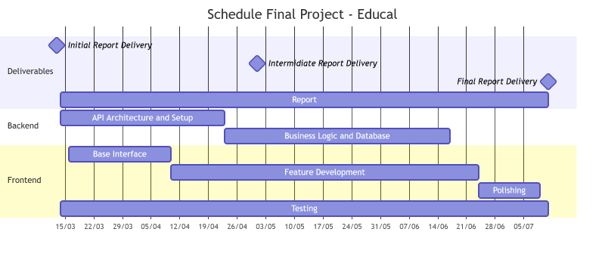
\includegraphics{./figures/schedule_gantt.png}}
\end{center}
\caption{Project schedule (Gantt chart).}\label{fig:schedule}
\end{figure}
